\documentclass{article}
\usepackage{graphicx} % Required for inserting images
\usepackage[a4paper, total={6in, 8in}]{geometry}
\usepackage{url}
\usepackage{hyperref}

\title{ArtBot: An Investigation into the Human Brain's Comprehension of Aesthetic Value}
\author{Anirdesh Shankar}

\begin{document}

\maketitle

\section{ArtBot}

ArtBot is a proposal and hypothetical machine learning model that will be designed to understand how humans value art and thus will facilitate the understanding of how human brains process art and understand aesthetic value. It will investigate why humans value certain kinds of things and what kinds of aspect create value in art. This machine learning model will be built using a neural network. The ML model will use the price of the artwork will be the labels and the artwork in an image format will the input to the model. Regression will be performed on the data set using the neural network in order to build a model that can tell us the relationship between different features of the image and how they influence the price. The price is a proxy measurement for the value we give a certain piece of artwork. Even though this is not the most accurate method of measuring value as aesthetic value is not always monetary, we can assume that it is an adequate proxy variable as something that has a greater impact on people will often resulting in them paying more for it or giving it a higher valuation. This project will mainly entail feature extraction. Through building and training a neural network, we can investigate the kinds of features that are most important in determining the output of the model. \newline 

This AI is meant to be able to tell us something about the way our brains process visual data like art and what makes our brain find something satisfying or aesthetically pleasing. Neural networks are chosen as they have a very good ability to process complex data and find patterns in them thereby allowing us to investigate implicit relationships between human valuation and the art that is valued. By using a model to bridge the input and output or here the visual stimulus which is the art and the aesthetic value we give it which is the price of the art, we can get an approximate understanding of the kinds of patterns of thinking our brains have when they interpret or look at art. The kinds of visual stimuli that make our brain think something is aesthetically pleasing. This AI is derived from the research methodology of trying to corroborate theories and models of human thinking in cognitive psychology through the use of computers. By modelling the stimuli and their response through a machine learning model that derives from biology, we can get an understanding of the kinds of features that influence our thinking. \newline

However, this AI might not yield concrete results or understanding in the exact way our brains think but the features extracted and the model trained in this regression task might allow us to get a better view of how our brains could process visual information and aesthetics. It will also allow us to understand the kinds of aspects of images and visual stimuli that make humans value something. On the other hand, this is a subjective question and not everyone thinks the same but the results of this ML experiment could yield in some sort of a model to investigate this idea through the use of computer modelling and experimentation. 

\section{Designing ArtBot}

The machine learning model will mainly use 3 different kinds of models. The first is a Convolutional Neural Network (CNN) in order to go from the one dimensional image data to the single value price data. This will use different neural network layers like a dense layer and a pooling layer to reduce the complexity of the image. A generative model will also be used to in order to do the same operation backwards. After learning the features that make a painting more pricey or less pricey, the machine learning model will be able to reproduce art in the same style using the features. This will allow us to get a better understanding of how a art of $x$ price would look as a means of understanding what kinds of things are aesthetic and not. Therefore a generative part of the model is necessary. One kind of technology that can be used for this is a transformer or a generative adversarial network. \newline 

Another machine learning technique that can be used to create ArtBot is unsupervised learning and especially multidimensional clustering. Each image can be put through a pooling layer and a sliding windows algorithm in order to create kernels that can then represent groups of pixels in a condensed form. This is one way to extract features from the image. These features along with the labels can be represented as data points on a higher dimensional hyperplane. An algorithm like k means clustering can find structure within this data in order to show which kinds of paintings are similar and whether they have the same price. This can help identify visual patterns in the way we value artworks. This can allow us to find features and structure in the data set through a different perspective. This method can help find similarities on different "dimensions". This could be kinds of colors used, the kinds of strokes used in different parts of the painting and the kinds of styles or combinations of lines which are all represented in the pixel data but unlabelled. They will also all be plotted on the axis of price to factor in the "value" of the painting. The graph below is a representation of how this could look in 3 dimensions, 2 dimensions of pixel values and 1 dimension of prices. \newline

\begin{figure}[htp]
    \centering
    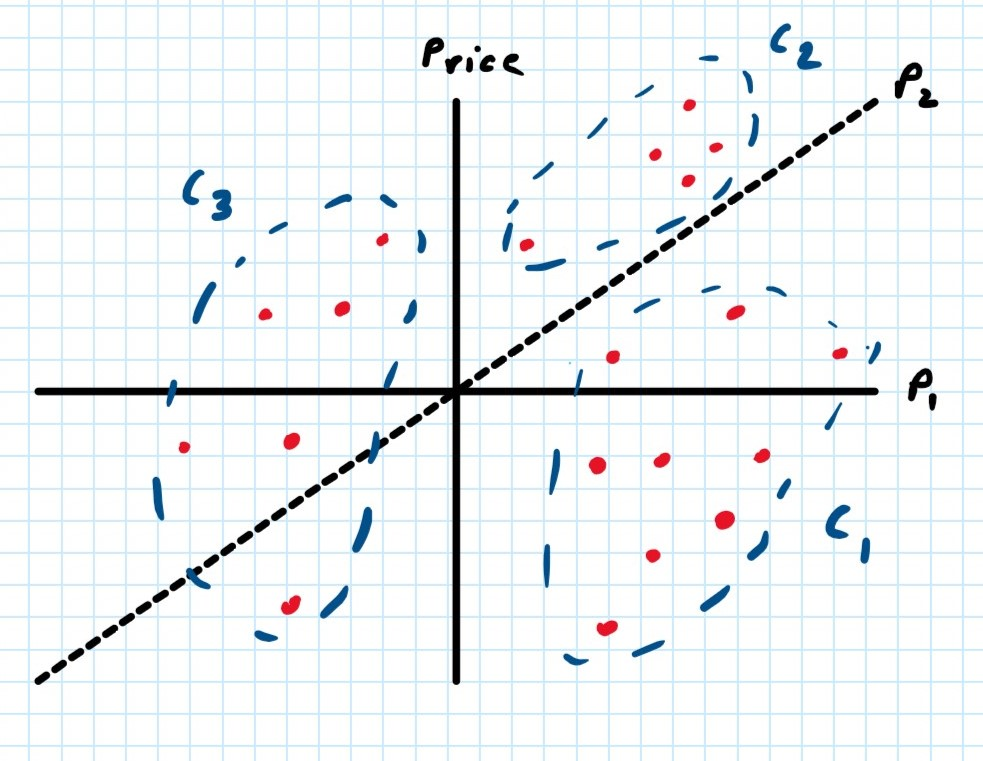
\includegraphics[width=9cm]{KMeans.jpg}
    \caption{Representation of unsupervised clustering in 3 dimensions}
    \label{fig:kMeans}
\end{figure}

The insights of these methods can be combined in order to yield a more general understanding of the data set and human cognition of aesthetics. The consistency of results can also be compared to see whether the same features that determine value from an art piece is the same. This could give more evidence to a general model for human aesthetic cognition existing. 

\subsection{Data and Pre-processing}

The data is one of the most important parts of training this AI. This is because, this AI learns its knowledge from data and not on its own exploration or through pre-programmed algorithms. This introduces a lot of both technical but also ethical considerations. The data can be sourced from the internet where different artworks are put up for sale. This means that the value of the artwork is directly proportional to how much a human values the piece. On average, it can be assumed that the more valued the piece, the more people bid on it so the more value people saw in it. However, not everyone bids in auctions therefore another label source can also be used where people are allowed to estimate the price they would pay for art in a survey format. This achieves the same outcome without the consideration of actions not being accessible to everyone. This is also a method of diversification. A combination of these data sources or a selection can be made after obtaining the data to analyze biases.

It is important that a wide range of pieces with a lot of diversity in color, style, time, setting and artist are chosen such that the data set is heterogeneous. This will allow for a more wider and less biased exploration. Furthermore, the data must be inclusive of all different kinds of art as aesthetic value is a very wide subject so inclusion is a must in order to ethically consider all kinds of "value". Like Watson, we need to curate the data in order for it to get a good understanding of the field. Therefore, the AI is reliant on human intervention and therefore is not truly independently intelligent. It still has bias however, this bias can be eliminated by being more deliberate in the choice of the data set. \newline

%  is the action format really the best value label?? replace the auction value label with a survey format value label??

There are also a few technical considerations in how the data is collected and processed. One problem is that lighting and resolution are different for every image therefore the images must be cropped and the resolutions must be corrected such that there is a standard brightness and resolution for all the pictures. If this is not done then it could result in biases in the results. The data must also be corrected for any external objects or frames which are not part of the artwork as this could alter the results. Finally, the data must also be put in a form which can be read in by the computer. In order to do this, the data comes in a $x \times y$ format with 3 channels of color data. This can be represented as a tensor in an array format with dimensions $x \times y \times 3$. The 3 is for the 3 RBG channels. This can then be flattened into a single dimensional array to feed into the neural network. However, a window layer can also be applied onto the image in order to pre process in order to extract features which will further help the model process the data more efficiently. This process is shown in Figure 2.

\begin{figure}[htp]
    \centering
    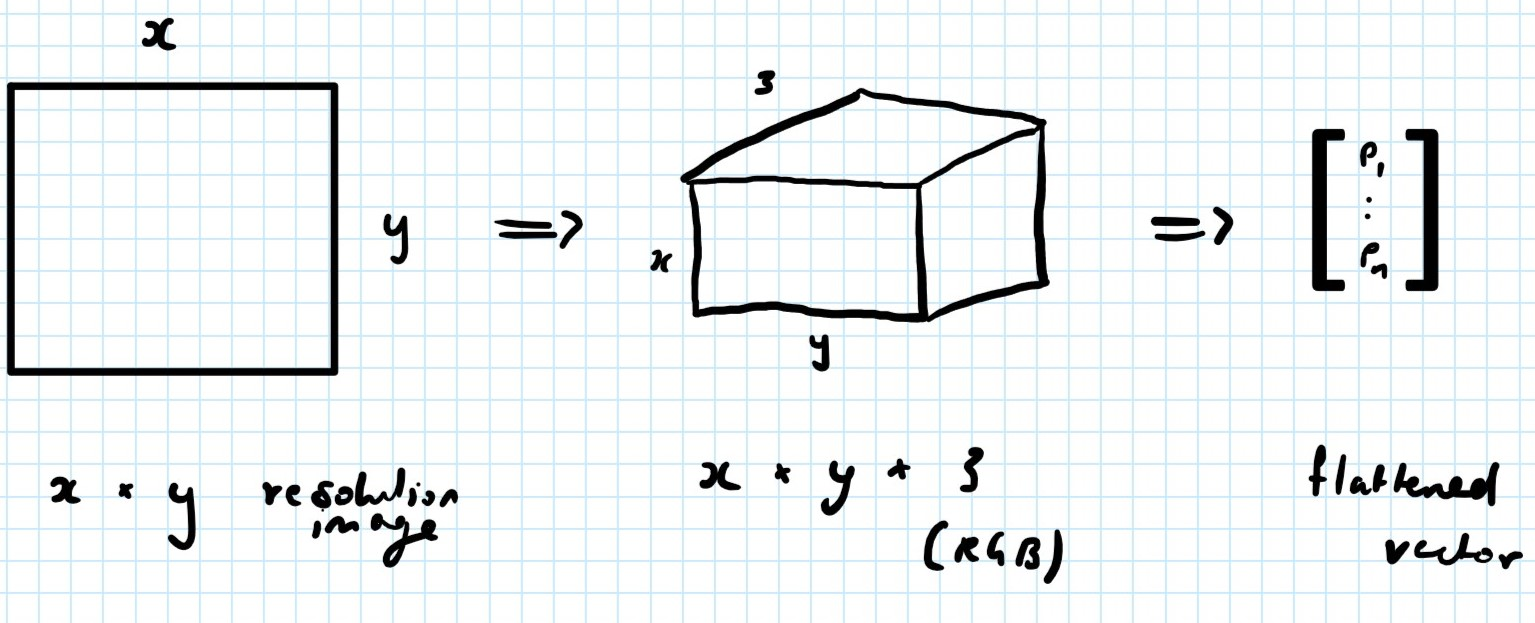
\includegraphics[width=11cm]{preprocessing.jpg}
    \caption{Schematic for Data Preprocessing}
    \label{fig:data}
\end{figure}

\subsection{Machine Learning Architecture}

The following is a high level schematic for how the different machine learning models could be designed. The relationship between the GAN and CNN can be thought of like a function and its inverse. The CNN goes from the image to a price and in the process extracts features whereas the GAN takes in an input as random noise and then generates pictures out of it. These two contrary methods can be used to check whether the same features are present in both methods as a means of checking whether aesthetic "value" is consistent and if this can be identified through different methods. 

\subsubsection{Convolutional Neural Network (CNN)}

A convolutional neural network is a method of using image data in order to perform regression or classification tasks. This is the exact problem that this AI is trying to solve. Namely, we want to convert from a picture of an art piece to a price which is a continuous variable therefore this is a regression task. A convolutions layer which is the central part of a CNN is a method of feature extraction from an image. The higher level idea is that you can take a window or a $n \times m$ frame of pixels called a kernel and then move it over the image. You can to a linear algebra operation on the matrix or kernel to transform the window into a singular number in order to extract more general and larger patterns in the image from single pixel values. \newline

The second part of the network is a pooling layer. This is a layer that basically reduces the resolution of the images in order to make the features or patterns more apparent and reduce the computational capacity. This allows the model to check for more general and robust features instead of proverbially being stuck in the smaller details of the image and over fitting. \newline

The network architecture proposed in Figure 3 is an implementation of this idea where the features are extracted using a convolutions layer and then they layers are pooled in order to extract the most important patterns and information from the image. The data is then flattened and then fed through a neural network with activation in order to transform the multi feature data into a single number or a price. One way that this process can be thought of is that the convolutional layer and the pooling layers transform the data and extract the higher level features. The next fully connected dense layers then find the relationships between the different features or kernels identified in the previous step. \newline

In order to train the model, a loss will be calculated from the predictions of the models which will be propagated through the neural network through back propagation. The loss will probably be a version of Mean Squared Error or Root Mean Squared Error as this problem is a regression task so finding the distance between the labels or ground truth which is the actual price and the predicted price is a good way of finding error. This error will then be minimized. Figure 3 shows a schematic for the CNN. 

% investigate the art itself or the way humans interact with the art?

\begin{figure}[htp]
    \centering
    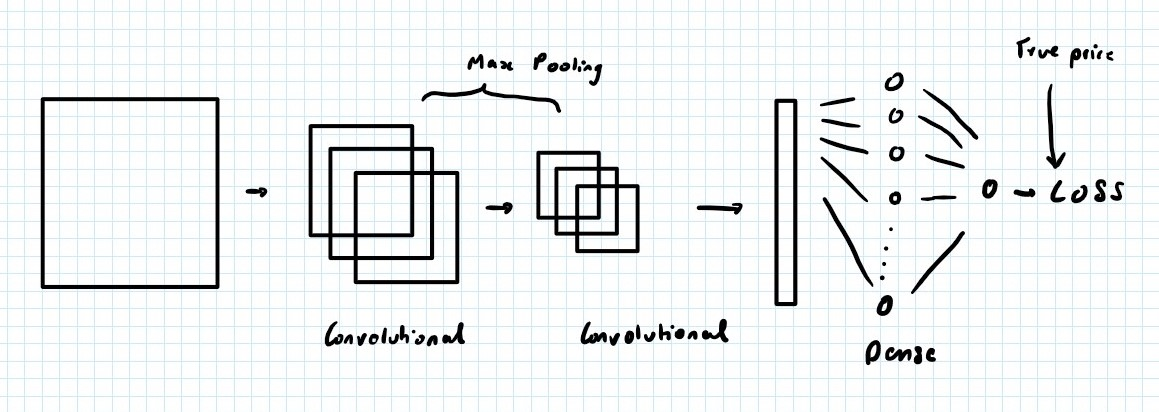
\includegraphics[width=11cm]{CONV.jpg}
    \caption{Network Archecture Draft for CNN}
    \label{fig:CNN}
\end{figure}

\subsubsection{Generative Adversarial Network (GAN)}

A Generative Adversarial Network is a combination of two different architectures of neural networks. They can be used to generate artwork in the style or similar to ground truths images that are fed to them. The whole model can be split up into two sections. The first is a generator. The generator basically build up an image from random noise. It taken convolutional layers and 
can use both CNN and unsupervised learning, generative models to generate results from the features it learns, use it as a means of producing new content that resembles the labels. The generator part of the network essentially takes in a random distribution of values in a vector format and then transforms it into an image. This is done through up sampling using convolutions. Basically it reshapes the random values into an image using a CNN. By updating the weights of the model to generate images in a certain way through calculating loss against the test data, it will produce better images. \newline   

On the other hand, the discriminator is a CNN that tries to output whether the image that the generator has made is real or fake by comparing it to real images. It basically does the inverse of the generator and uses a CNN to go from the image to a binary classification of whether the image is true or false. Here truth corresponds to if the generated images matches up with the test set through the calculation of a loss using binary cross entropy. The combination of the discriminator and the generator which are both updated using the loss creates an "adversarial" relationship. Or in other words, the generator tries to trick the discriminator to classify its generated images as real. Both networks keep improving and trying to get better than each other thereby applying pressure for the generator to improve its weights and biases to produce better images and vice versa for the discriminator. \newline 

In the case of ArtBot, the GAN will be trained on multiple data sets. The data sets will range from the most valued or priciest artworks to the least pricey artworks in order to train the GAN to generate images similar to these artworks. This is a way of basically training the GAN to adopt a style of creating artworks therefore allowing us to investigate different aesthetic elements or styles of artworks in different price ranges.  Even though art could hold a greater meaning than price and its value is not always monetary, we can understand what makes certain art more valuable than others by asking a computer to learn different styles and aspects of art pieces that are valued different amounts. A suggested architecture for the GAN is shown in Figure 4. \newline  

If the GAN and the CNN end up having the same kinds of features and their results end up correlating we can see that there is a certain general aesthetic value in art. One way to check this is to use a similar idea to the GAN. One can feed the generated images from the GAN to the CNN in order to check its value and see whether this matches other artworks that are similarly priced. If this is the case then the machine learning model is able to understand where value comes from in artworks. \newline

%One way to relate the CNN from the previous section with the GAN is to use the trained features from the CNN and itegrate them into the random state which the generator produes from. This will allow the genreator to produce in a certain prederminted style.

\begin{figure}[htp]
    \centering
    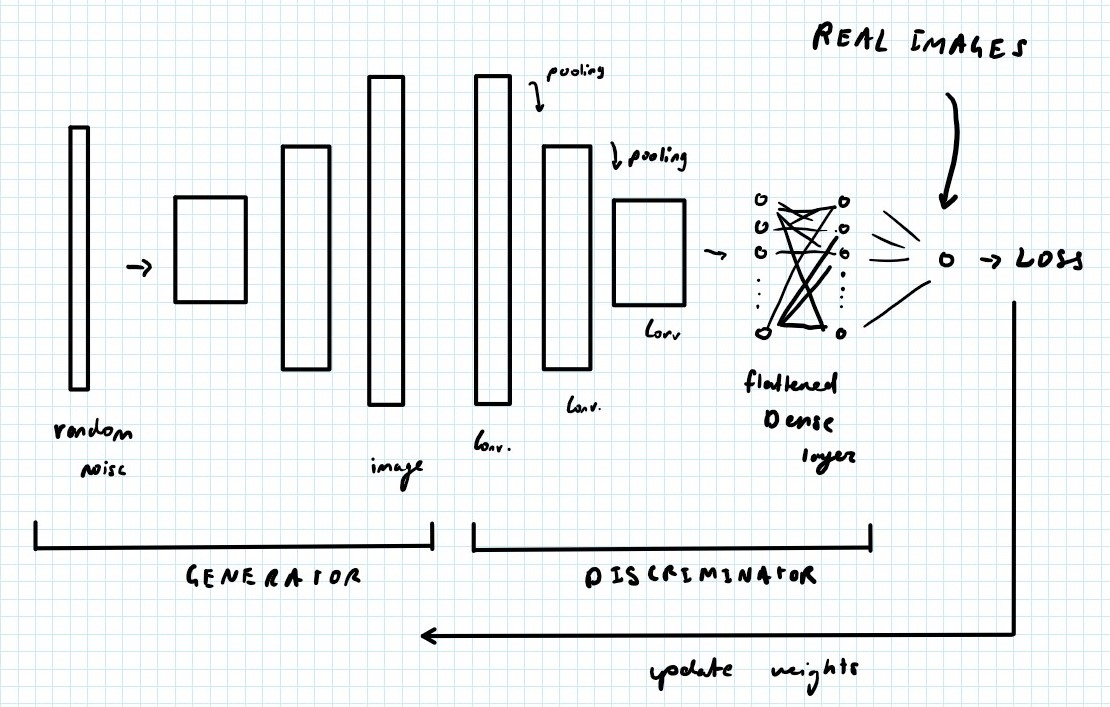
\includegraphics[width=10cm]{GAN.jpg}
    \caption{Example Network Architecture for GAN}
    \label{fig:data}
\end{figure}

\subsection{ General Training Scheme}

The testing scheme in general will be through splitting the data set into a train and test data set. The train data set will be used to train the model over epochs and calculate the loss or divergence from the ground truth in order to update the model. The model then will be tested on a smaller test data set to observe its performance on unseen data. The ideal behaviour of the model is that the CNN is able to accurately guess the price from the image and it has been trained in such a way that the features it has extracted clearly demonstrates patterns in the images with the same prices. For the GAN, it should be able to produce high quality images and it should be trained to an extent where the images it produces is extremely similar to the real artworks to a human viewer. This is similar to a Turing test but for visual stimuli. \newline 

On a larger level, the AI will be trained constantly and iteratively making its knowledge dynamic. The data set will constantly change and not be absolute. One method to do this is to use artworks and predict their prices in real time as artworks change in price and new artworks are being sold in order to make the model relevant to changes in the market and thus in the taste of humans. The data set itself will be updated and changed. Furthermore, another method of making its knowledge dynamic is to use an ensemble method. \newline 

Another method of making the AI dynamically gain new knowledge about the world is to generate more real time features of measuring the tastes of different people.  \emph{A method of doing this is to constantly ask people to enter a value of money to see how much they value the art piece} and take the average of this as the average price or value. This will help factor in more perspectives and give a more general label which will make the model more representative. Furthermore, this can also be changed over time which will factor the change in tastes over time. In terms of the GAN, we can also factor in \textbf{\emph{dynamic user input}}. The discriminator can be made to factor in another loss function where the truth ranking comes from humans along with the discriminator network in order to factor in the tastes of humans and their opinions on how much value they would value or pay for the generated art. This is a more realistic loss function that models the taste of humans. This can also be changed over time when retraining the GAN thus allowing it to update its weights to be more representative of the current valuation of humans. But the limitation is that "value" cannot be really quantified in a completely representative manner but here the price is an adequate estimate for the value of something, especially if the \emph{price is agreed upon and averaged over a population}. \newline  

Different CNN's and GAN's can be trained using different price ranges of artworks and then their predictions on an artwork can be joined together to make the model more specific and accurate. Instead of needing to deal with over fitting in a single model by adding too many layers or features, multiple models can be trained with data that is segregated by prices. For example one CNN would be trained to recognize mainly artwork that costs a lot and another would mainly recognize artworks that has prices in a mid level based on the price distribution. However, each model would also be fed artworks at different prices in order to create diversity in its predictions. Then the CNN predictions would be combined to produce the most likely price. This is a way of making the knowledge more dynamic as it allows for the model to consider many options and take into consideration a wider range of "perspectives" or differently trained models. This results in a greater diversity of conclusions and more confident results. 
 
%what kind of loss function? how will you optimize?

%constant and iterative training process that will be dynamic based on changes in price of works of art and it can be used to predict the value of a work of art and see how well it did in real time. It can also be trained on a matrix of value feaures like on a scale of 1 to 10 how mcuh something was lciked and for eahat reason, addition of mroe features over time. It adapts and the dataset changes and it corrects itself as poeple assign it value or not

%It will genarate works of art and then people can rank the valeu fo teh waork and art and it will update it weihgts based on this after the intial price training 

\section{Is ArtBot Intelligent?}

According to Searle this AI might not be intelligent at all. However, this is not a drawback as this AI is meant to be a model that is trained to convert from input to output. What is important in this AI is the model itself. The weight, biases and features that the model extract can tell us a lot about how aesthetics are processed and converted into value. It can give us an insight into the things our brains look for when they see something aesthetically pleasing. Therefore, the intelligence of this AI comes from its ability to recognize complex patterns and find relationships in data that are not obvious to humans. Therefore this is more like an intelligent tool than a smart intelligence itself. It is reliant on human filtering and cannot think and correct itself on its own. Therefore it is not intelligent in the way humans are. However, we can using a Turing like test to check whether this AI can show intelligence in its field or objective function which is to find value from art. The images it generates and the value it assigns paintings can be compared with human recognition like a random trial where humans identify the value of paintings and guess whether the computer generated paintings are a lot of value or not. If the AI passes this test, then we can to an extent conclude that it has "learnt" what it means to have monetary value in art or has reached knowledge in its niche or its objective function. This does not mean that it has hard coded knowledge as it is able to extrapolate so it is completely a computer program that follows instructions but at the same time it does not have the capability to understand how or why to produce art. Therefore it can never be intelligent in the domain of artistic knowledge. However, it might have gained a lot of knowledge about patterns in art creation and human perception of value through being trained with a data set. However, all its knowledge can be altered and its perception can be changed through different design choices and parameter tunings like choosing a different loss function therefore its knowledge is not extremely dynamic. Its knowledge is not also extremely accurate or in a broader sense valid as it is based of price data and a limited dataset which does not accurately represent all the different kinds of value and different perspectives people can have on art pieces and thus is biased. Therefore its knowledge might be biased and not accurate. However, it can be used as a higher level proxy model to understand general trends in how humans associate value to art so to a very low extent it is knowledgeable. Another argument that can be made is that a technique like neural networks are sub-symbolic methods do not really contain codified knowledge. This is because the AI knows things in the forms of weights and biases. It knows that a certain combination of numbers results in the ability to interpret data and extrapolate results from but the reason behind why these numbers work or what these numbers really are remain unknown. In contrary, a symbolic or logical model knows exact what each variable means and the logical relationship between variables therefore it "understands" the results it produces. This means that the AI does not "know" its own knowledge. Therefore, when thinking about knowledge in relation to computer models that are statistical and not symbolic or logical, we must ask the question, "Does the ability to know constitute the knowledge itself?"



\begin{thebibliography}{9}

\bibitem{ImgGen}
 Yalçın, Orhan G. “Image Generation in 10 Minutes with Generative Adversarial Networks.” \emph{Medium}, Towards Data Science, 12 Jan. 2023, https://towardsdatascience.com/image-generation-in-10-minutes-with-generative-adversarial-networks-c2afc56bfa3b. 

\bibitem{googleGAN}
“Background: What Is a Generative Model?” \emph{Google}, Google, 18 July 2022, https://developers.google.com/machine-learning/gan/generative.

\bibitem{CNN}
Pokhrel, Sabina. “Beginners Guide to Understanding Convolutional Neural Networks.” \emph{Medium}, Towards Data Science, 20 Sept. 2019, \href{https://towardsdatascience.com/beginners-guide-to-understanding-convolutional-neural-networks-ae9ed58bb17d#:~:text=A%20convolution%20layer%20transforms%20the,a%20kernel%20(or%20filter).&amp;text=A%20kernel%20is%20a%20small,convolution%20matrix%20or%20convolution%20mask} 

\bibitem{Convolutions}

Rohrer, Brandon. “How Do Convolutional Neural Networks Work?” Table of Contents, 18 Aug. 2016, \href{https://e2eml.school/how_convolutional_neural_networks_work.html#:~:text=CNNs%20compare%20images%20piece%20by,two%2Ddimensional%20array%20of%20values.}

\end{thebibliography}

\end{document}
